\section{Aufbau}\label{sec:aufbau}
\begin{figure}[H]
    \centering
    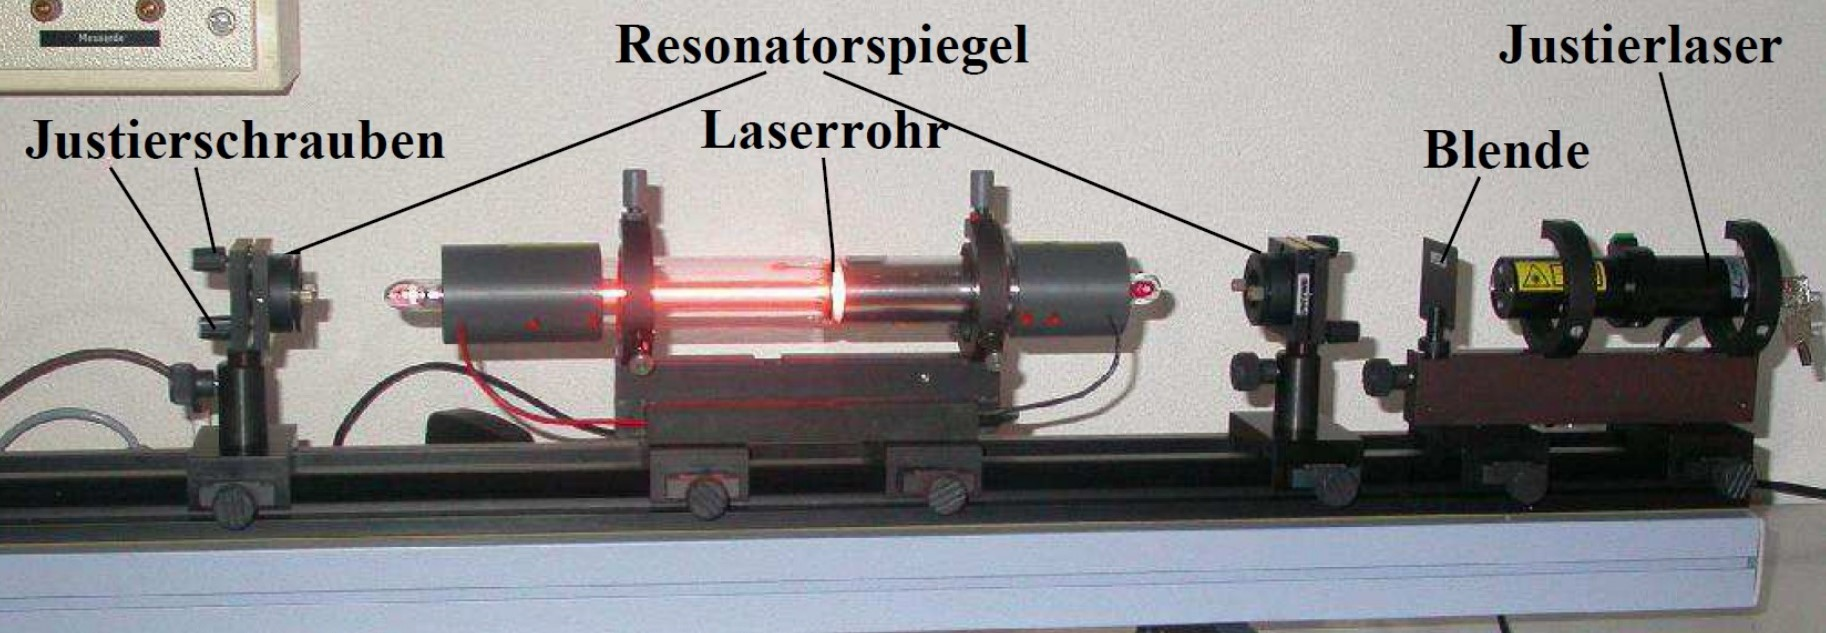
\includegraphics[width=0.6\textwidth]{grafiken/aufbau.jpg}
    \caption{Aufbau des Experiments.\cite{V61}}
    \label{fig:aufbau}
\end{figure}
Der Aufbau ist in \autoref{fig:aufbau} zusammengefasst. Zu den bereits erwähnten Bauteilen kommt nun noch ein Justierlaser, der als Hilfe dient, um den Helium-Neon-Laser zum Lasen zu bringen.
Es stehen mehrere Spiegel zur Verfügung - diese sind in \autoref{fig:spiegel} dargestellt.
\begin{figure}[H]
    \centering
    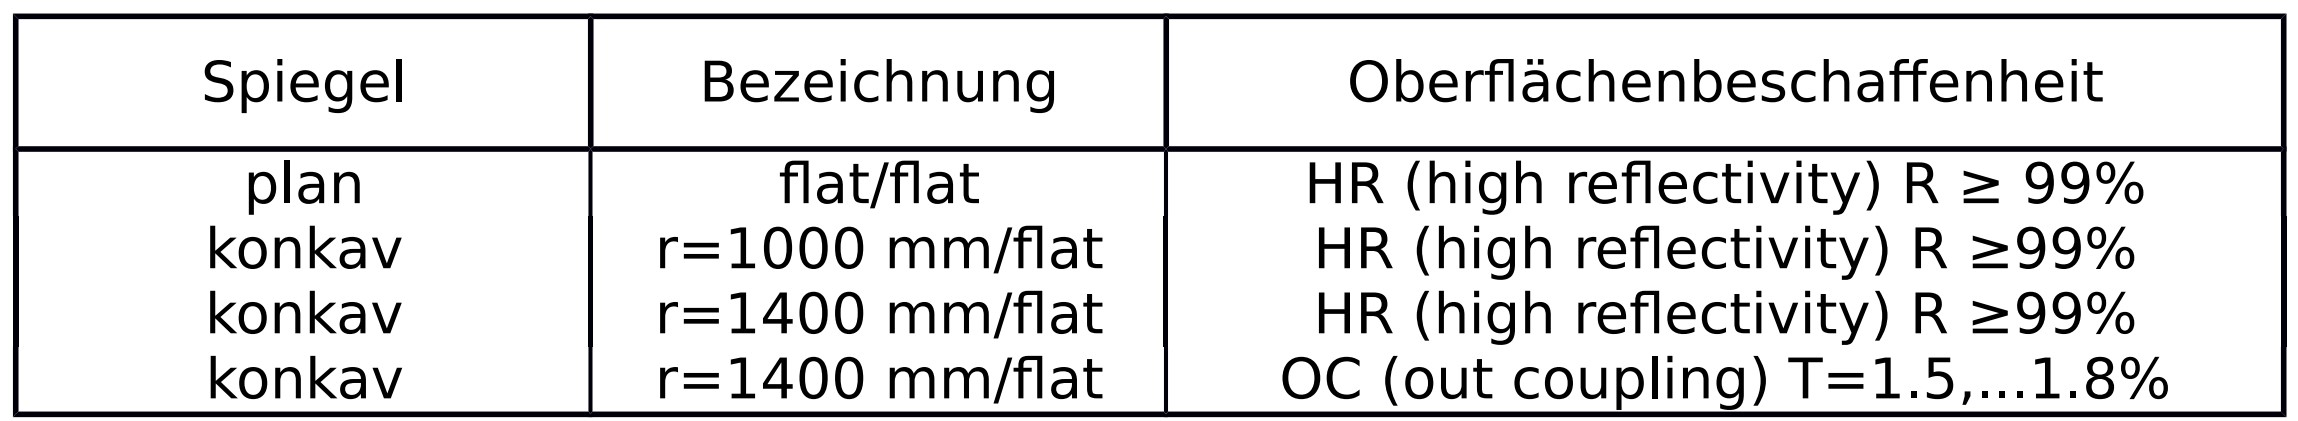
\includegraphics[width=0.6\textwidth]{grafiken/spiegel.jpg}
    \caption{Verschiedene Spiegel.\cite{V61}}
    \label{fig:spiegel}
\end{figure}

\section{Durchführung}
\label{sec:Durchführung}
In diesem Versuch muss der Laser justiert werden, die Stabilitätsbedingung überprüft, die Transversalmoden und Longitudinalmoden bestimmt, die Polarisation des Lasers untersucht und die Wellenlänge des Lasers bestimmt werden.
\subsection{Justage des Lasers}
Zuerst werden alle nötigen Bauteile auf die Schiene montiert und der Justierlaser eingeschaltet. Die Resonatorspiegel werden so eingestellt, dass der Rückreflex des Justierlasers
auf das Fadenkreuz der Justierblende fällt. Danach müssen die Spiegel so lange feinjustiert werden, bis der Laserbetrieb einsetzt.
\subsection{Stabilitätsbedingung}
Die Stabilitätsbedingung wird überprüft, indem der Abstand der Spiegel variiert wird. Diese werden so lange verschoben, bis der Laserbetrieb nicht mehr möglich ist. Das wird für 
zwei verschiedene Spiegelkombinationen durchgeführt.
\subsection{Transversalmoden}
Die Transversalmoden werden bestimmt, indem eine Photodiode senkrecht zur Ausbreitungsrichtung des Lasers bewegt wird. Die Intensität wird dabei aufgenommen und die Intensitätsverteilung
bestimmt.
\subsection{Longitudinalmoden}
Ein Oszilloskop wird an den Photodiodenstrom angeschlossen. Dann können die Frequenzpeaks der Longitudinalmoden bestimmt werden. Das wird für verschiedene Resonatorlängen durchgeführt.
\subsection{Polarisation}
Die Polarisation des Lasers wird untersucht, indem ein Polarisationsfilter in den Strahlengang gebracht wird. Der Photodiodenstrom wird in Abhängigkeit des Winkels des Filters aufgenommen.
\subsection{Wellenlänge}
Die Wellenlänge des Lasers wird bestimmt, indem ein Gitter in den Strahlengang gebracht wird. Dann wird der Abstand der Beugungsmaxima auf einem Schirm gemessen. Dies wird für vier verschiedene
Gitter mit unterschiedlichen Gitterkonstanten durchgeführt.

\newpage